%!TEX root = ./main.tex

\section[Phase]{The Signal Is a Wave}

% SECTION TIMING: 16:00--24:00 (2 frames). The pivot of the lecture: stop reading
% how LOUD the wave is, read WHERE IN ITS CYCLE it is. One figure sells it; the
% second figure immediately shows the catch (wrapping) so the two rulers that
% follow are motivated, not announced.

% Teaching note (210 s): trace the figure with a finger. Amplitude decays -- that
% was RSSI. Underneath, the phase rotates one full turn per wavelength. At 5 GHz a
% wavelength is 6 cm, so one degree of phase is 0.17 mm of path. The complex number
% h is what the Wi-Fi card computes for every subcarrier and every antenna just to
% decode the packet (Class 8) -- the industry calls the collection CSI.
\begin{frame}{The signal is a wave; the phase is a ruler}
  \vspace{0.2em}
  \centering
  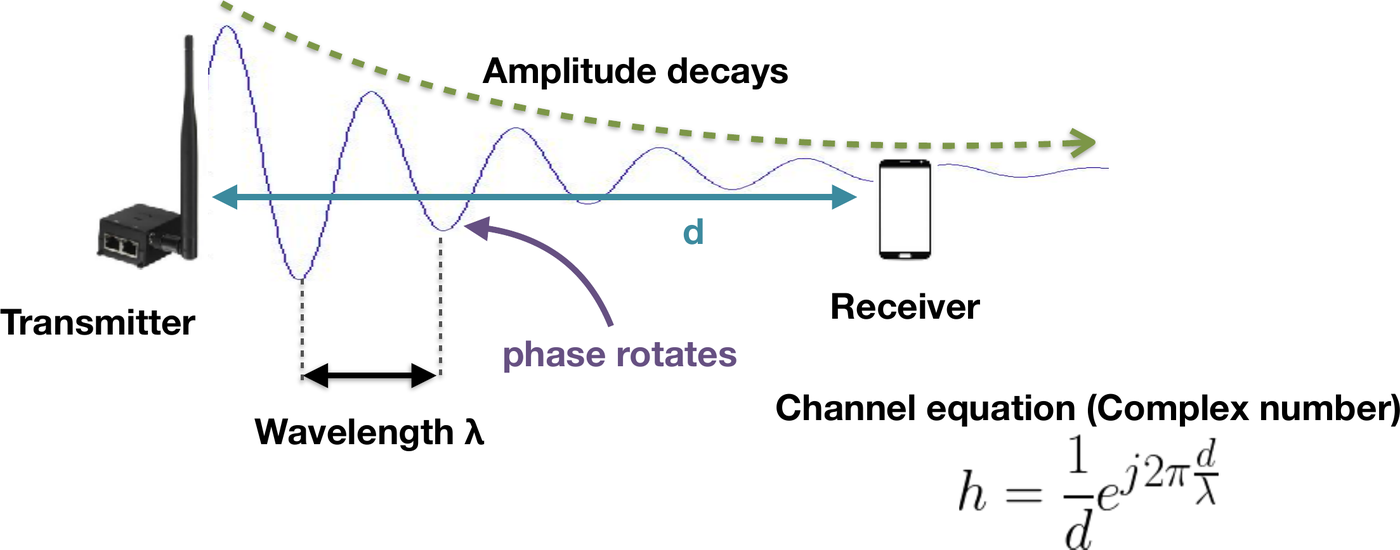
\includegraphics[width=0.92\textwidth]{figure/mit_wave.png}

  \vspace{0.3em}
  \raggedright
  {\small
   \begin{itemize}\itemsep2pt
     \item Amplitude decays --- that was RSSI. \textbf{Phase turns $360^\circ$
       every wavelength.}
     \item 5 GHz: $\lambda = 6$ cm, so $1^\circ$ of phase $\approx$ 0.17 mm of path.
     \item The card already computes $h$ per subcarrier, per antenna, to decode
       (Class 8): that is \textbf{CSI}.
   \end{itemize}\par}
  \glossline{CSI = Channel State Information: the $h$ values the receiver estimated
    from the packet preamble}
  \source{https://www.mit.edu/~fadel/courses/MAS.s60/materials/Lec2-localization-2022.pdf}{Figure: MIT MAS.S60 Lecture 2}
\end{frame}

% Teaching note (180 s): the catch. The red ticks are every moment the phase reads
% the same value: one period apart, 0.4 ns, 12 cm. A phone 5 m away has turned 87
% full times; the AP sees only the last fraction of a turn. So a single phase reading
% is worthless -- and the whole rest of the lecture is two ways of reading a
% DIFFERENCE instead: two antennas (angle) or two frequencies (distance).
\begin{frame}{\ldots but the ruler has no numbers on it}
  \vspace{0.2em}
  \centering
  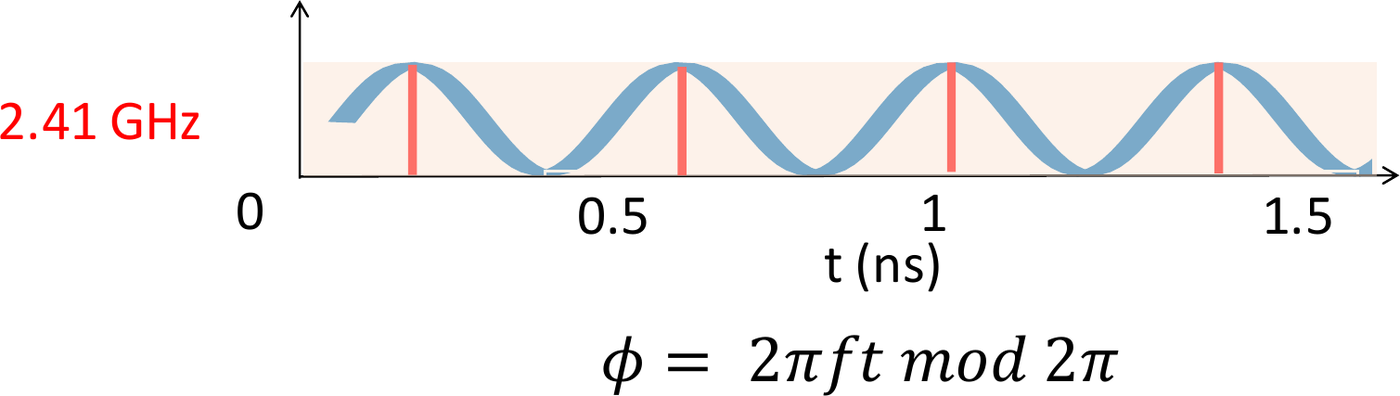
\includegraphics[width=0.8\textwidth]{figure/ch_one_freq.png}

  \vspace{0.2em}
  {\small Every red tick looks identical to the receiver. A 5 m path has turned
   $\approx 87$ times; you see only the leftover fraction.\par}

  \vspace{0.4em}
  \takeaway{You cannot read \emph{one} phase. You can read the \textbf{difference}
    between two:\\
    two \textcolor{ranblue}{antennas} $\to$ \textbf{angle}; \quad
    two \textcolor{coreorange}{frequencies} $\to$ \textbf{distance}.}
  \source{https://www.usenix.org/conference/nsdi16/technical-sessions/presentation/vasisht}{Figure: Vasisht, Kumar \& Katabi, Chronos talk, NSDI 2016}
\end{frame}
